%preprocessing
\subsection{Preprocessing}

La strategia di preprocessing dei dati è essenziale nel caso in cui si abbiano features non rilevanti per l'output, troppe features rispetto al numero di samples, range di valori del dataset estremamente grandi, quantità di samples troppo grande per essere computata in tempi ragionevoli. 
\newline Prima di effetture il vero preprocessing, ho creato delle funzioni che mi permettessero di cambiare i valori dei dati nei range consigliati dai medici. Per questo motivo ho usato delle mie funzioni "custom" per poter discretizzare i dati entro i range prescelti dai medici.
\newline Per quanto riguarda il target non ho effettuato nessun tipo di operazione in quanto era già convertito in 4 valori numerici.
\newline Le strategie più utilizzate, quando si hanno valori compresi tra range molto ampli, sono quelle di standardizzazione e normalizzazione dei dati.
Standardizzare i dati vuole dire portare i valori di una variabile aleatoria X con varianza \begin{math}\sigma\end{math} e media \begin{math}\mu\end{math} ad una variabile Z, con distribuzione standard, ovvero media zero e varianza uno:
\begin{equation}
    Z=\frac{X-\mu}{\sigma}
\end{equation}
Questo procedimento è utilizzato per riportare alcuni valori molto grandi di features diverse nelle stesso range. Così facendo non ci saranno valori con un peso maggiore rispetto ad un altro.
La normalizzazione segue lo stesso concetto, tuttavia la formula che la descrive è diversa e la nuova variabile "vivrà" in un range tra 0 e 1:
\begin{equation}
    Z=\frac{X-min}{max-min}
\end{equation}
dove \textit{min e max} sono rispettivamente il minimo e il massimo valore del dominio dove vivono i valori della feature stessa.
\newline Per la mia tiplogia di problema, non ho voluto appositamente usare questi due metodi di preprocessing poichè non l'ho ritenuto necessario. Nessuno dei valori delle feature, essendo discretizzati precedentemente, necessita di essere standardizzato o normalizzato nè ci sono valori molto grandi. Per di più ci sono valori discreti di molte features, che assumono valore o 0 o 1: applicando questi metodi i loro valori sarebbero stati gli stessi, sprecando solamente delle risorse computazionali. 


Per quanto concerne il mio datset ho voluto utilizzare due strategie:
\begin{itemize}
    \item Rimozione delle features non utili alla classificazione sulla base dell'EDA
    \item Usare il metodo di selezione di k features con K-Best
\end{itemize}

\newline Come rilevato precedentemente (vedi fig. \ref{fig:distr_features_1}) nel dataset è presente una feature con sempre lo stesso valore, ovvero RNA base. Per questa ragione ho eliminato questa feature. Si è passati quindi da 28 features a 27 features. Questo tipo di operazione di features selection è stata effettuata "manualmente" osservando i risultati dell'EDA. Questi tipi di features selection basati sull'EDA sono noti come \textbf{filter methods}. Ho deciso di mantere anche le altre features con bassa varianza poichè questi valori potrebbero essere necessari ai fini della classificazione essendo valori estratti da referti medici. Inoltre testando i modelli ed eliminando queste features, le perfomance dell'algoritmo calavano notevolmente, in particolare l'accuracy. Così ho deciso di seguire un'altra strada per un'ulteriore features selection senza però applicarlo manualmente. Questa operazione è stata effettuata scartando la colonna corrispondente alla feature "RNA Base" che tramite la funzione di VarianceThreshold con parametro di input di default "threshold"=0. Ciò sta ad indicare che questa funzione eliminerà le features con varianza nulla come appunto RNA Base. 
\newline Non avendo forti correlazioni tra le features e l'output target ho proceduto come segue.
\newline Mi sono preoccupato di selezionare le k features più rilevanti, usando un metodo di preprocessing chiamato "K-Best". Questo metodo seleziona le k migliori features basandosi sulla varianza delle features e quanto queste influiscono sull'uscita. Per determinare quale sia il valore ottimale di k, ho testato un range tra 12 e 27 (di k). Il test è stato effettuato per ognuno dei 2 algoritmi selezionati per la classificazione (KNN e Decision Tree ), riportando il k che migliora l'accuracy. Da ciò è emerso che il valore k ottimale per K-nearest neighbors è 24 mentre, per il Decision Tree è 19, vedi fig.\ref{fig:features_selectionKNN}
\newline Il funzionamento di KBest è semplice: prendere in input il training set e "fittarlo" in base all'output riferito allo stesso train set e selezionare le k features per le quali si ha uno "score" elevato. Questo score può essere misurato attraverso diversi test, tra i quali \begin{math}\textbf{\chi^{2}}\end{math} da me utilizzato. Questo test misura la dipendenza tra una variabile (in questo caso la feature) e la variabile target, escludendo le features che sono più indipendenti dall'output e quindi inutili per la classificazione. 
Selezionare meno features comporta uno sforzo computazionale drasticamente minore per gli algoritmi di Machine Learning, con lo svantaggio di sacrificare alcuni dati. 
Riporto in una tabella le features selezionate per ogni algoritmo, tab. \ref{tab:features_selected}

\begin{table}[ht]
\centering
\begin{tabular}{@{}lcc@{}}
\toprule
   & \multicolumn{1}{l}{\textbf{Number of features selected}} & \textbf{Features selected}                                                                                                                                                                                                                                                                                                                                                                              \\ \midrule
\multicolumn{1}{|l|}{\textit{For KNN}}           & \multicolumn{1}{c|}{24}                                  & \multicolumn{1}{c|}{\begin{tabular}[c]{@{}c@{}}'Age', 'Gender', 'BMI', 'Fever',\\  'Nausea or Vomiting', 'Headache ', 'Diarrhea '\\  'Fatigue \& generalized bone ache' 'Jaundice ',\\  'Epigastric pain ', 'WBC',\\  'RBC', 'HGB', 'Plat', 'AST 1',\\  'ALT 12', 'ALT 24', 'ALT 36', 'ALT 48',\\  'ALT after 24 w', 'RNA 12',\\  'RNA EOT', 'RNA EF',\\  'Baseline histological Grading'\end{tabular}} \\ \midrule
\multicolumn{1}{|l|}{\textit{For Decision Tree}} & \multicolumn{1}{c|}{19}                                  & \multicolumn{1}{c|}{\begin{tabular}[c]{@{}c@{}}'Age', 'Gender', 'BMI' 'Fever',\\  'Nausea or Vomiting', 'Headache ', 'Diarrhea '\\  'Fatigue \& generalized bone ache', 'Jaundice ',\\  'Epigastric pain ', 'WBC',\\  'HGB', 'Plat' ,'ALT 36' ,'ALT after 24 w',\\ 'RNA 12', 'RNA EOT', 'RNA EF',\\  'Baseline histological Grading'\end{tabular}}                                                      \\ \bottomrule
\end{tabular}
\caption{ Le features selezionate per i due algoritmi attraverso KBest}
\label{tab:features_selected}
\end{table}
\begin{figure}[H]
    \centering
    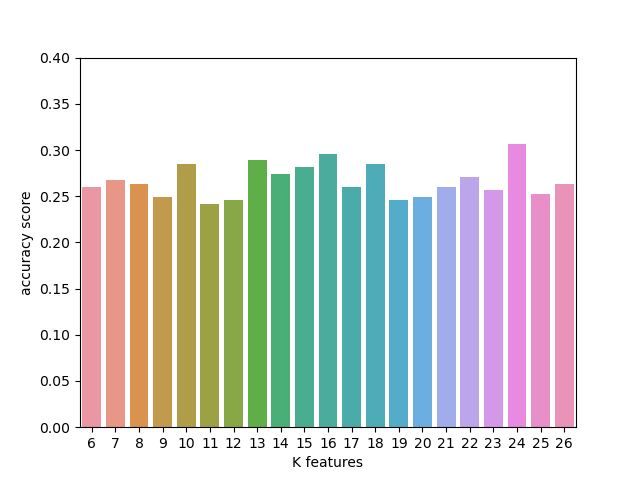
\includegraphics[width=0.5\columnwidth]{figures/KBEST_KNN.png}
    \caption{Accuracy al variare di K in KNN, con K: numero di features}
    \label{fig:features_selectionKNN}
\end{figure}

\begin{figure}[H]
    \centering
    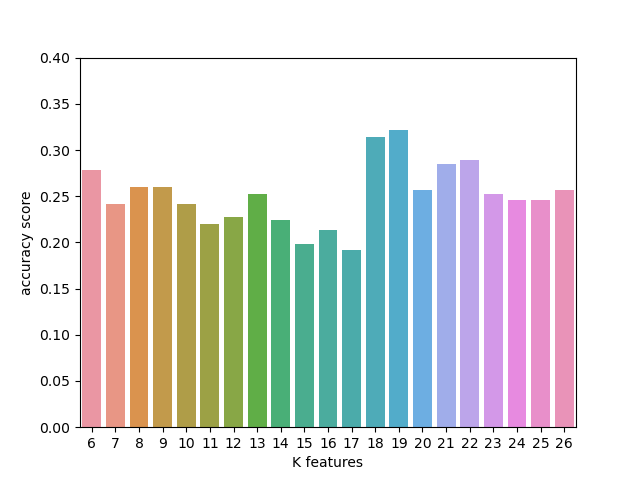
\includegraphics[width=0.5\columnwidth]{figures/KBestDT.png}
    \caption{Accuracy al variare di K in Decision Tree, con K: numero di features}
    \label{fig:features_selection_DT}
\end{figure}


